In this section, the layer is described in some detail in terms of its specific subsystems. Describe each of the layers and its subsystems in a separate chapter/major subsection of this document. The content of each subsystem description should be similar. Include in this section any special considerations and/or trade-offs considered for the approach you have chosen.

\subsection{Acoustic Array}
The acoustic array will consist of a hexagonal printed circuit board with six microphones located at each point of the hexagon. Internally the board will contain the audio to digital converter and be capable of processing the microphone inputs from the array and forwarding that information to a digital component for processing. These requirements are meant by a COTS device called ReSpeaker, which will be the component used to meet these requirements. The subsystem will detect audio inputs from the environment and forward the raw analog audio data to the ADC for processing.

\begin{figure}[h!]
	\centering
 	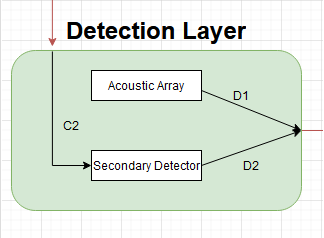
\includegraphics[width=0.50\textwidth]{images/detection}
 \caption{Acoustic Array}
\end{figure}

\subsubsection{Assumptions}
The ReSpeaker will detect across all six microphones and information will be compiled and properly forwarded to the ADC

\subsubsection{Responsibilities}
The subsystems sole purpose is to process raw audio data from the surrounding environment and compile it into a usable data stream. Each microphone works in tandem with the others to generate positional data, then forwards this information to the ADC to process and push further along the pipeline.

\subsubsection{Subsystem Interfaces}

\begin {table}[H]
\caption {Subsystem interfaces} 
\begin{center}
    \begin{tabular}{ | p{1cm} | p{6cm} | p{3cm} | p{3cm} |}
    \hline
    ID & Description & Inputs & Outputs \\ \hline
    \#RS01 & ReSpeaker Microphone Array & \pbox{3cm}{Microphone 1 \\ Microphone 2 \\ Microphone 3 \\ Microphone 4 \\ Microphone 5 \\  Microphone 6} & \pbox{3cm}{Compiled Audio Data to ADC}  \\ \hline
    \#RS02 & Power Supply & \pbox{3cm}{Power In} & \pbox{3cm}{N/A}  \\ \hline
    \end{tabular}
\end{center}
\end{table}

\subsection{ODAS Algorithm}
ODAS is an open source software developed for taking in multiple audio data sources and compiling it into usable data streams. For the purposes of the ARGOOSE system, ODAS will utilize a modified sourcing code to locate the sound of drones that are detected within the area of operation. At default, ODAS detects raw sounds and locations based off of the ReSpeaker array. This information is compiled and displayed on the software to pinpoint location and event data. Data streams will come in from the ADC on detected sound patterns, will be identified and manipulated by ODAS and then forwarded on to the Raspberry pi controller to display and interpret relevant data.

\begin{figure}[h!]
	\centering
 	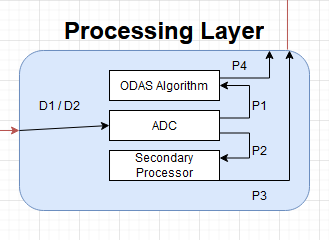
\includegraphics[width=0.50\textwidth]{images/processing}
 \caption{Example subsystem description diagram}
\end{figure}

\subsubsection{Assumptions}
ODAS algorithmic data processing will accurately detail drone detection and forward data streams that are relevant and interpretable by the Raspberry Pi.
Information received from the ADC will be in a format that is accurately analyzable by the ODAS algorithm.

\subsubsection{Responsibilities}
ODAS is responsible for generating the positional and occurrence data from the raw data stream of the ADC. It is the key component is generating the sample necessary for the controller to determine when and where drone detections should occur.

\subsubsection{Subsystem Interfaces}

\begin {table}[H]
\caption {Subsystem interfaces} 
\begin{center}
    \begin{tabular}{ | p{1cm} | p{6cm} | p{3cm} | p{3cm} |}
    \hline
    ID & Description & Inputs & Outputs \\ \hline
    \#RS01 & ODAS Algorithm & \pbox{3cm}{ADC Data Stream} & \pbox{3cm}{Compiled Detection Data to Controller}  \\ \hline
    \end{tabular}
\end{center}
\end{table}

\subsection{Subsystem 3}
Repeat for each subsystem

